% TeX eps-loader file generated by stoch_simul.m (Dynare).
% 28-Dec-2024 22:44:26
 
\begin{figure}[H]
\centering 
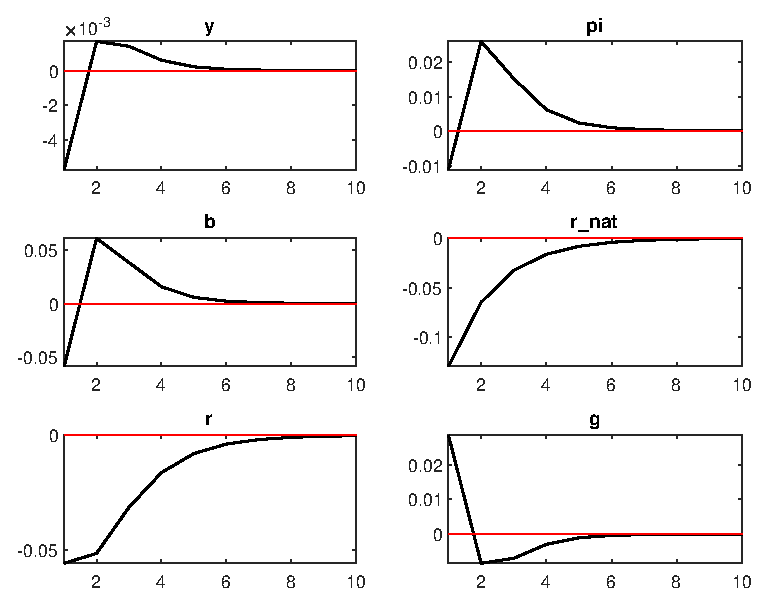
\includegraphics[width=0.80\textwidth]{nash/graphs/nash_IRF_eps_a}
\caption{Impulse response functions (orthogonalized shock to ${\varepsilon^a}$).}
\label{Fig:IRF:eps_a}
\end{figure}
 
\begin{figure}[H]
\centering 
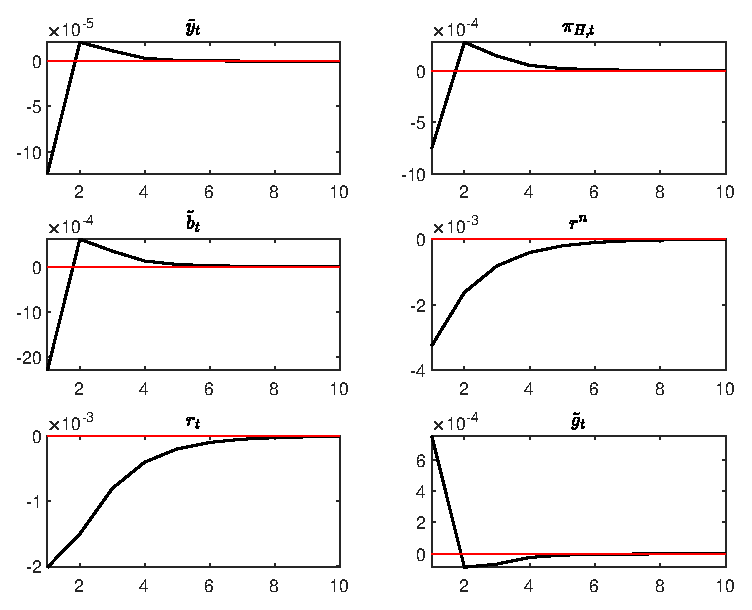
\includegraphics[width=0.80\textwidth]{nash/graphs/nash_IRF_eps_c_star}
\caption{Impulse response functions (orthogonalized shock to ${\varepsilon^c}$).}
\label{Fig:IRF:eps_c_star}
\end{figure}
 
\begin{figure}[H]
\centering 
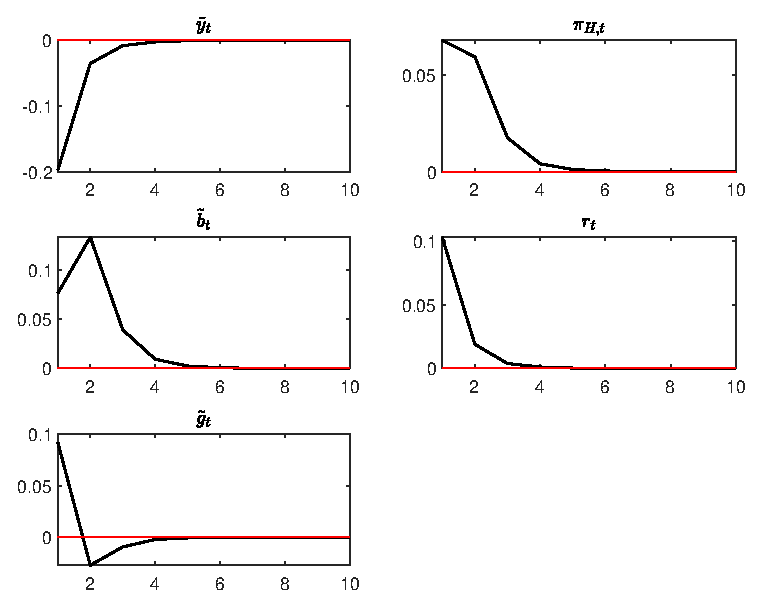
\includegraphics[width=0.80\textwidth]{nash/graphs/nash_IRF_eps_pi}
\caption{Impulse response functions (orthogonalized shock to ${\varepsilon^{\pi}}$).}
\label{Fig:IRF:eps_pi}
\end{figure}
 
\begin{figure}[H]
\centering 
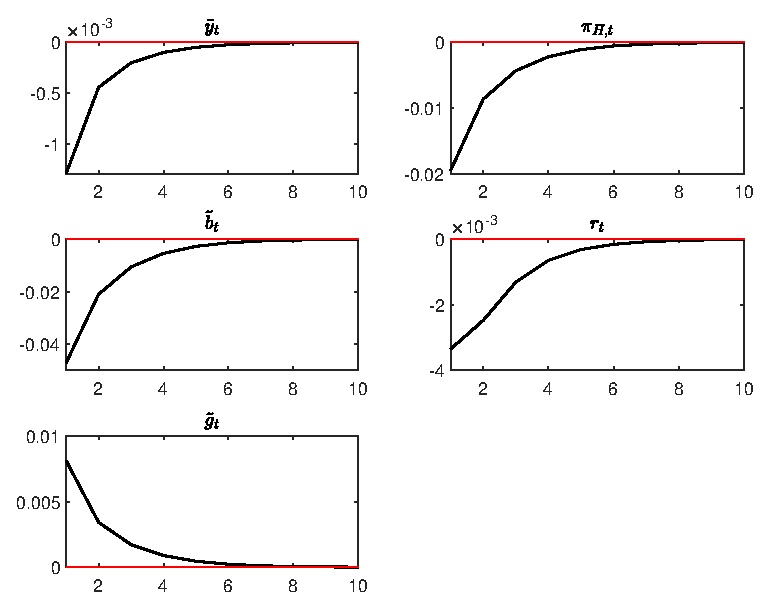
\includegraphics[width=0.80\textwidth]{nash/graphs/nash_IRF_eps_r}
\caption{Impulse response functions (orthogonalized shock to ${\varepsilon^{r}}$).}
\label{Fig:IRF:eps_r}
\end{figure}
 
\begin{figure}[H]
\centering 
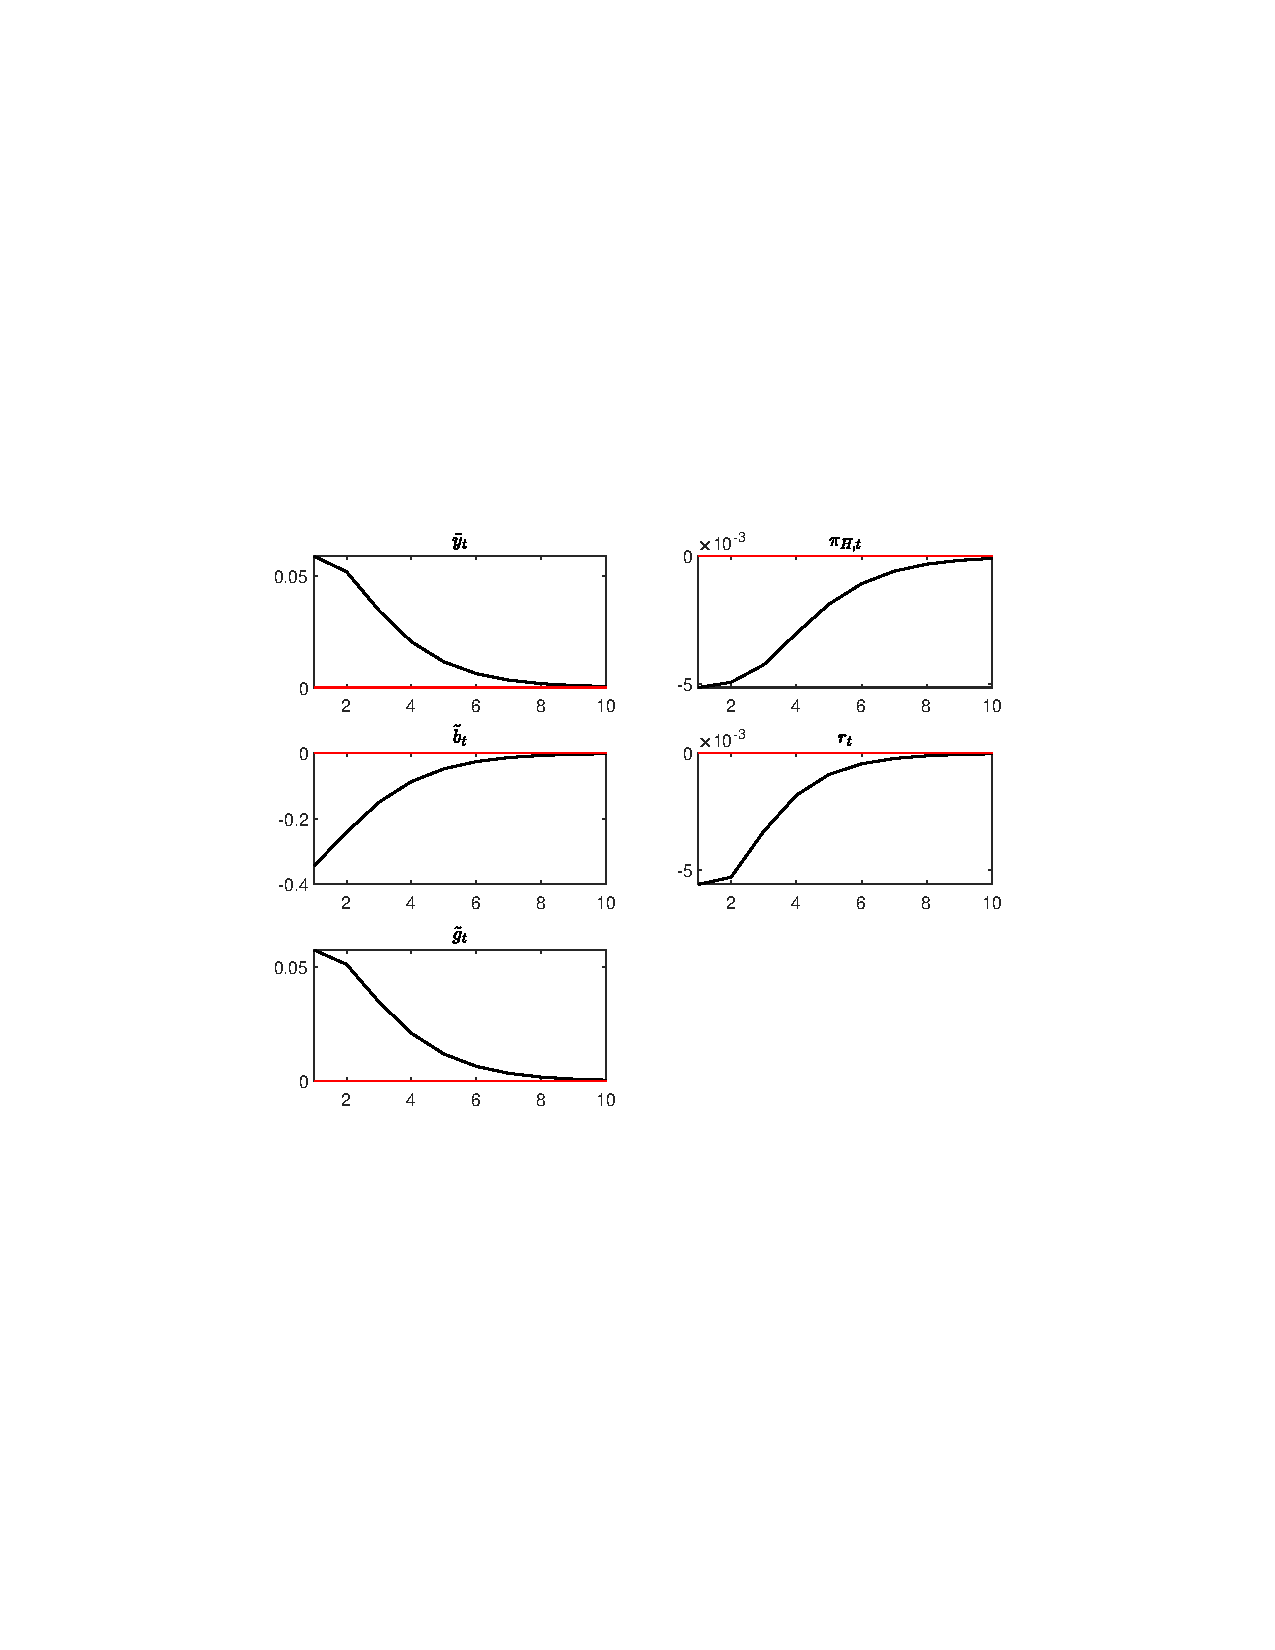
\includegraphics[width=0.80\textwidth]{nash/graphs/nash_IRF_eps_g}
\caption{Impulse response functions (orthogonalized shock to ${\varepsilon^{g}}$).}
\label{Fig:IRF:eps_g}
\end{figure}
 
 
% End Of TeX file. 
